%%%%%%%%%%%%%%%%%%%%%%%%%%%%%%%%%%%%%%%%%%%%%%%%%%%%%%%%%%%
% --------------------------------------------------------
%     BIBLIOGRAPHY WITH BIBLATEX IN EXTERNAL EDITORS
% --------------------------------------------------------
% If the bibliography does not show up, try running the 
% 'tau.cls' and 'tau.bib' file with biber from the 
% MikTeX console or your preferred LaTeX distribution to 
% generate the auxiliar files and (re)run the main.tex.
% --------------------------------------------------------
%%%%%%%%%%%%%%%%%%%%%%%%%%%%%%%%%%%%%%%%%%%%%%%%%%%%%%%%%%%
% --------------------------------------------------------
%					  FOR SPANISH BABEL
% --------------------------------------------------------
% \usepackage[spanish,es-nodecimaldot,es-noindentfirst]{babel}
% --------------------------------------------------------
%%%%%%%%%%%%%%%%%%%%%%%%%%%%%%%%%%%%%%%%%%%%%%%%%%%%%%%%%%%

\documentclass[10pt,a4paper,twoside]{tau}
\usepackage[english]{babel}
\usepackage{tauenvs}
\usepackage{xcolor}
\renewcommand{\vec}[1]{\mathbf{#1}}
\renewcommand{\d}{\text{d}}
%----------------------------------------------------------
% TITLE
%----------------------------------------------------------

\title{Image Classification Based On Three-Layer Neural Network}

%----------------------------------------------------------
% AUTHORS, AFFILIATIONS AND PROFESSOR
%----------------------------------------------------------

\author[]{Xiang Zheng, 21307110169}

%----------------------------------------------------------

\affil[]{School of Data Science, Fudan University}

%----------------------------------------------------------
% FOOTER INFORMATION
%----------------------------------------------------------

\institution{}
\ftitle{}
\date{}
\etal{}
\course{Computer Vision}

%----------------------------------------------------------
% ABSTRACT
%----------------------------------------------------------

\begin{abstract}    
    Welcome to tau ($\tau$) \LaTeX\ class for making academic articles and lab reports. In this example template, we will guide you through the process of using and customizing this class to your needs. For more information of this class check out the appendix section. There, you will find snippets codes that define key aspects of the template, allowing you to explore and modify them.
\end{abstract}

%----------------------------------------------------------

\keywords{\LaTeX\ class, lab report, academic article, tau class}

%----------------------------------------------------------

\begin{document}
		
\maketitle
\thispagestyle{firststyle}
\tauabstract
%----------------------------------------------------------

\section{Introduction}

\taustart{I}n this project, we aim to develop and train a fully connected neural network to classify images from the Fashion-MNIST dataset. The Fashion-MNIST dataset, curated by Zalando, comprises a collection of grayscale images representing various fashion items, along with corresponding labels indicating their respective categories. With 60,000 training examples and 10,000 test examples, this dataset serves as a standard benchmark for evaluating machine learning algorithms in the context of fashion image classification.

The neural network architecture we will employ consists of three linear layers, which will be trained to learn meaningful representations from the input images and make accurate predictions about their corresponding classes. Throughout this project, we will explore different components of the neural network, including activation functions, loss functions, and training strategies, to optimize its performance on the Fashion-MNIST dataset.

The remainder of this report is structured as follows: Section 2 provides the downloading the pre-process method of the Fashion-MNIST dataset. Section 3 delves into the specifics of the neural network architecture, detailing the design choices for its components. Section 4 outlines the training process, including the selection of hyper-parameters and evaluation metrics. In Section 5, we evaluate the trained model on the test dataset and present visualizations to assess its effectiveness. Finally, Section 6 offers concluding remarks and discusses potential avenues for future research and improvement.

\section{Dataset}

Having already covered the dataset's characteristics earlier, we'll now delve straight into the downloading and preprocessing steps. Utilizing the Python library \texttt{urllib}, we'll fetch the data from its \href{https://github.com/zalandoresearch/fashion-mnist}{official website} and organize it into a dictionary containing images and labels. Each numpy array representing a grayscale image will be reshaped into the format $(1, 28, 28)$ to maintain consistency with their original shapes.

\section{Model}

A standard linear layer neural network comprises three main components: the input layer, hidden layers, and output layer. The transition between the input (hidden) layer and hidden layers can be described as a \texttt{LinearActivation} layer, while the transition between the hidden layer and output layer involves a \texttt{Linear} layer along with a \texttt{loss} function. Other parameters like \texttt{reg} and \texttt{weight\_scale} also influence the performance of the model.

Before delving into the discussion of our model, it's essential to establish the key notations utilized throughout this report. Let $N$ represent the batch size, indicating the number of samples processed in each training or inference iteration. $D$ denotes the flattened dimension of the image, symbolizing the size of the image vector after flattening. $H_1, H_2, \cdots, H_n$ refer to the dimensions of the hidden layers within the neural network architecture. Finally, $C$ signifies the output dimension, representing the number of classes in the classification task.

\subsection{Linear Layer}

Consider the first linear layer as an illustration. The forward pass can be concisely expressed as:

\begin{equation}
    \vec{Y} = \vec{X}\vec{W} + \vec{b} \tag{3.1.1}
\end{equation}

Here, $\vec{Y} \in \mathbb{R}^{N \times H_1}$, $\vec{X} \in \mathbb{R}^{N \times D}$, $\vec{W} \in \mathbb{R}^{D \times H_1}$, and $\vec{b} \in \mathbb{R}^{H_1}$. It's worth noting that \texttt{numpy} broadcasts $\vec{b}$ to fit into the computation. Hence, I represent $\vec{b}$ as a vector to maintain alignment with my code implementation. Also, please note that we need to 'cache' the current values of $\vec{X}$ and $\vec{W}$ for the backward pass.

Regarding the backward pass, the input of the backward function is \texttt{dout} and \texttt{cache}, where \texttt{dout} represents the gradient at $\vec{Y}$ with shape $(N, H_1)$. Taking derivatives with respect to $\vec{X}$ and $\vec{W}$, we obtain:

\begin{equation}
    \d\vec{X} = \d\vec{Y} \cdot \vec{W}^{\top} \tag{3.1.2}
\end{equation}
\begin{equation}
    \d\vec{W} = \vec{X}^{\top} \cdot \d\vec{Y} \tag{3.1.3}
\end{equation}
For bias $\vec{b}$, the derivative involves summing \texttt{dout} over the first dimension. 

You can observe that the shapes of these matrices match perfectly. The same technique can be applied to other following linear layers. Feel free to refer to my code in \texttt{linear\_layer.py} to see the details of implementation.


\subsection{Activation Functions}

When it comes to activation functions, they all perform an element-wise operation on the given matrix. There are several commonly used types of activation functions, including \texttt{ReLU}, \texttt{Tanh}, and \texttt{Sigmoid}. Let's introduce each of them individually.

\subsubsection{ReLU}

For the forward pass, ReLU is expressed as:
\begin{equation}
\vec{Y'} = \max(\vec{Y}, \vec{0}) \tag{3.2.1}
\end{equation}
For the backward pass, it's:
\begin{equation}
\d\vec{Y} = \max(\d\vec{Y'}, \vec{0}) \tag{3.2.2}
\end{equation}

\subsubsection{Tanh}

The mathematical expression of the hyperbolic tangent function, Tanh, is:
\begin{equation}
\tanh{x} = \frac{e^{2x} - 1}{e^{2x} + 1} \tag{3.2.3}
\end{equation}
Taking the derivative with respect to $x$, we get:
\begin{equation}
\frac{\partial \tanh{x}}{\partial x} = \frac{4}{(e^{2x}+1)^2} = 1 - \tanh^2{x} \tag{3.2.4}
\end{equation}

The forward and backward pass follows directly from the above equations:
\begin{equation}
\vec{Y'} = \tanh{\vec{Y}} \tag{3.2.5}
\end{equation}
\begin{equation}
\d\vec{Y} = \d\vec{Y'}\cdot(1 - \tanh^2\vec{Y}) \tag{3.2.6}
\end{equation}

\subsubsection{Sigmoid}

Let's denote the sigmoid function as:
\begin{equation}
\sigma(x) = \frac{1}{1 + e^{-x}} \tag{3.2.7}
\end{equation}
Taking the derivative with respect to $x$, we obtain:
\begin{equation}
\frac{\partial\sigma(x)}{\partial x} = \frac{e^{-x}}{(1 + e^{-x})^2} = \sigma(x)(1 - \sigma(x)) \tag{3.2.8}
\end{equation}
Then, the forward and backward pass of the sigmoid function are:
\begin{equation}
\vec{Y'} = \sigma(\vec{Y}) \tag{3.2.9}
\end{equation}
\begin{equation}
\d\vec{Y} = \d\vec{Y'}\cdot \sigma(\vec{Y}) (1 - \sigma(\vec{Y})) \tag{3.2.10}
\end{equation}

\subsection{Loss Function}

The loss function plays a crucial role in training a neural network as it quantifies the discrepancy between the predicted output and the actual target. Here, I'll implement the \texttt{cross\_entrophy}. Since this is a multi-class classification task, the CE is slightly different from the binary case.

For traditional binary cross entropy, the loss function is

\begin{equation}
    \text{loss}(\vec{y}, \vec{\hat{y}}) = -\frac{1}{N} \sum_{i=1}^{n}y_i
    \log(\hat{y}_i) + (1 - y_i) \log(1 - \hat{y}_i) \tag{3.3.1}
\end{equation}

where $y_i$ can only take the value of 0 or 1. However, this is not appropriate in multi-class classification.

To compute the loss function in the forward pass of the neural network, we'll first apply the softmax function to the raw output scores to obtain the predicted probabilities for each class. The softmax function is defined as:

\begin{equation}
\text{softmax}(\vec{x})_i = \frac{e^{x_i}}{\sum_{j=1}^{C} e^{x_j}} \tag{3.3.2}
\end{equation}

where $\vec{x}$ is the vector of raw output scores, and $C$ is the number of classes. This function ensures that the predicted probabilities are normalized and sum up to $1$ for each sample. Besides, the 'shifted x' method is used here to avoid overflow.

Once the softmax probabilities are computed, the cross-entropy loss can be calculated using the true labels and the predicted probabilities. The cross-entropy loss is defined as:

\begin{equation}
\text{CE} = -\frac{1}{N} \sum_{i=1}^{N} \sum_{s=1}^{C} t_{i,s} \log(f(s)_i) \tag{3.3.3}
\end{equation}

where $N$ is the number of samples, $C$ is the number of classes, $t_{i,s}$ is the true label for the $i$-th sample and $s$-th class (which is $1$ if the sample belongs to class $s$ and $0$ otherwise), and $f(s)_i$ is the predicted probability for the $i$-th sample belonging to the $s$-th class. Hence the loss can be further simplified as
\begin{equation}
    \text{CE} = -\frac{1}{N} \sum_{i=1}^{N} t_i \log(f(s)_i) \tag{3.3.4}
\end{equation}

In the backward pass, we'll need to compute the gradient of the loss function with respect to the raw output scores. This involves subtracting the true labels from the softmax probabilities, resulting in the gradient matrix. The gradient can be calculated as:

\begin{equation}
\frac{\partial \text{CE}}{\partial \mathbf{x}} = \frac{1}{N} (\text{softmax}(\mathbf{x}) - \mathbf{t}) \tag{3.3.5}
\end{equation}
and it's implemented in Python code as
\begin{center}
\begin{lstlisting}[language=Python,
        stringstyle=\color{green},
        numbers=none,
        keywordstyle=\color{purple},
        keywords={np, arange, sum, copy, exp}
    ]
# probs denotes the softmax result
probs = np.exp(log_probs)
loss = -np.sum(log_probs[np.arange(N), y])
loss /= N
dx = np.copy(probs)
dx[np.arange(x), y] -= 1
dx /= N
\end{lstlisting}   
\end{center}


\subsection{Other Parameters}

In addition to the model architecture, such as linear and activation layers, neural networks often involve hyper-parameters such as \texttt{hidden\_dims}, \texttt{reg}, and \texttt{weight\_scale}. 

For \texttt{hidden\_dims}, it determines the size of the hidden layers. Here, I've chosen the empirically recommended values $[128, 64]$.

\texttt{reg} is a regularization parameter that helps prevent overfitting by penalizing large weights in the model. In the next section, I'll discuss how grid search is used to find the best value for \texttt{reg}.

For the initial scale of the weight matrix, a commonly recommended value is 0.01. This value provides a good starting point for weight initialization, ensuring that the network begins training with reasonable weights.

\section{Train}

Now that we've covered the details of the Fully Connected Neural Network (FCNN) model in the previous section, let's delve into the training procedures. We'll begin by introducing some update rules, followed by a sanity check of the \texttt{Solver} on a small dataset to ensure its functionality. Subsequently, we'll conduct training for 2000 iterations for each configuration to identify the best configuration. Finally, the model will undergo training based on the optimal parameters for a significantly larger number of iterations to achieve the best results.


\subsection{Update Rule}

For update rules, I have provide four commonly used methods: stochastic gradient descent (SGD), SGD with momentum, Adam, and RMSprop. The mathematical explanation and some intuitions will be given below, while the experiment results of comparison of these four update rules will be defer to section 4.3.

\subsubsection{SGD}

The vanilla stochastic gradient descent is
\begin{equation}
    \vec{w} = \vec{w} - \texttt{lr} \cdot\d \vec{w} \tag{4.1.1}
\end{equation}
where the default value of \texttt{lr}(learning rate) is $1e^{-3}$.

\subsubsection{SGD Momentum}

For stochastic gradient descent with momentum, the update rule is 
\begin{equation}
    \vec{v} = \texttt{momentum} \cdot\vec{v} - \texttt{lr} \cdot\d\vec{w} \tag{4.1.2}
\end{equation}
\begin{equation}
    \vec{w} = \vec{w} + \vec{v} \tag{4.1.3}
\end{equation}
where $\vec{v}$ denotes the velocity. The empirical default values for \texttt{lr} and \texttt{momentum} are $1e^{-3}$ and $0.9$, respectively.

The advantages of SGD with momentum includes:
Momentum is faster than stochastic gradient descent the training will be faster than SGD. Local minima can be an escape and reach global minima due to the momentum involved. They'll be validated in the following experiments.

\subsubsection{Adam \& RMSprop}
Adam and RMSprop can be viewed as applying first-order and second-order normalization on the weight vector $\vec{w}$ respectively. These update rules are more complex compared to the ones discussed above. For a detailed explanation, please refer to the code implementation in \texttt{optimization.py}.


\subsection{Sanity Check}

For the sanity check, we trained the model using the first 500 samples of the training dataset for 2000 iterations. We set the hidden dimensions as $[128, 64]$ and used the \texttt{ReLU} activation function. The training results are depicted in Figure \ref{fig:sanity-check}:

\begin{figure}[hbp]
    \centering
    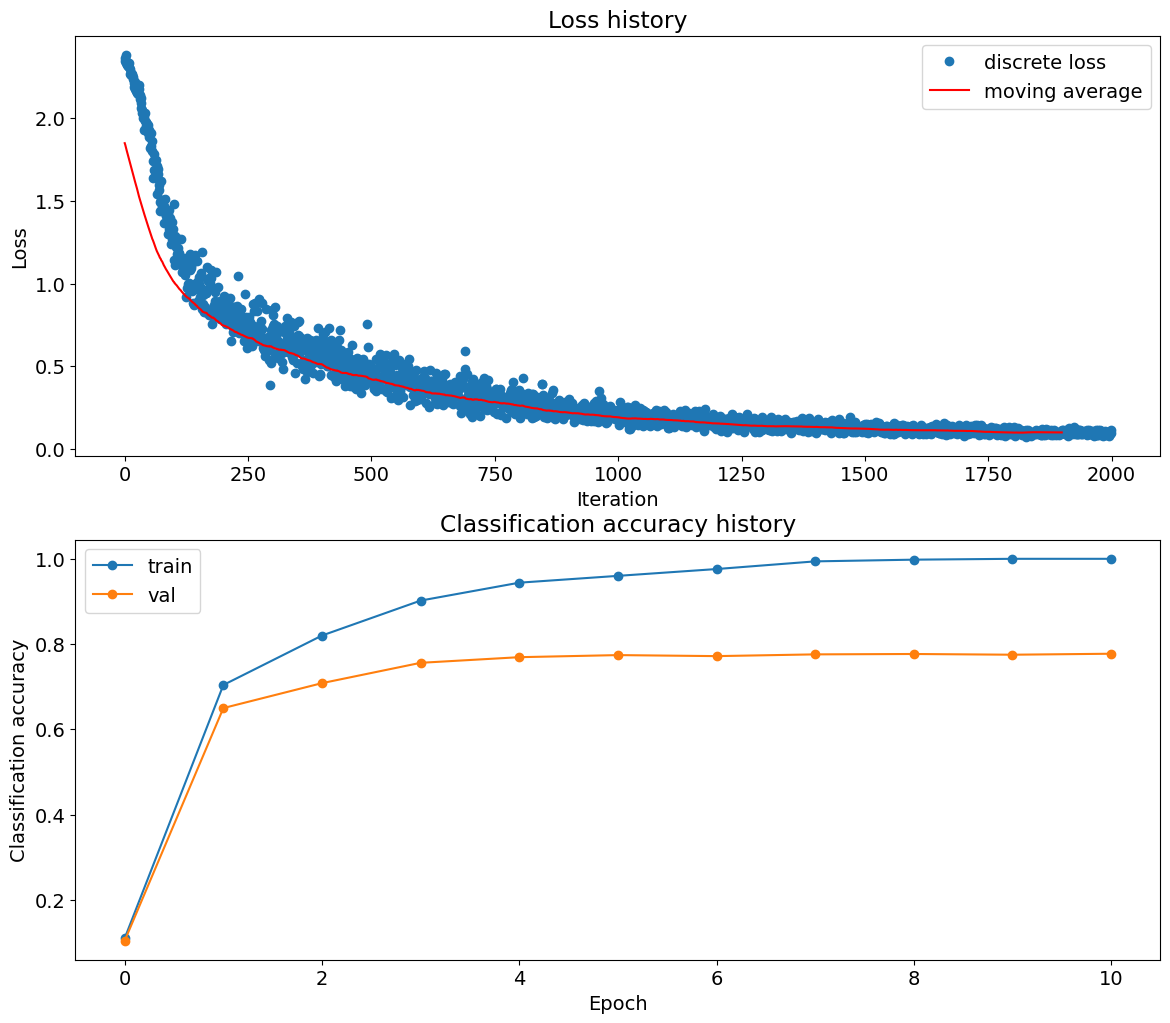
\includegraphics[scale=0.3]{images/sanity_check.png}
    \caption{Training on the Small Dataset}
    \label{fig:sanity-check}
\end{figure}

After 9 epochs of training (approximately 1800 iterations), the model achieved perfect accuracy on the training dataset, while the validation (testing) accuracy plateaued around 0.75. This indicates that our model is capable of overfitting the small subset of training data well, ensuring its availability for use. Now, let's proceed to fine-tune the model using the entire training dataset to find the best parameters.


\subsection{Search Best Configuration}

The process of searching the best configuration is divided into three subsections. First, the model will undergo training using 9 different combinations of activation functions while keeping other parameters constant, which can be seen as a greedy search. Subsequently, we will implement a grid search method to find the best hyper-parameters \texttt{reg}, \texttt{learning\_rate}, and \texttt{lr\_decay}. Finally, we will experiment with 4 different update rules mentioned in section 4.1.2 and compare their performance.


\subsubsection{Activation Function}

As discussed in Section 3.2, we offer three commonly used activation functions: \texttt{ReLU}, \texttt{Tanh}, and \texttt{Sigmoid}. In a three-layer neural network, there are two layers for activation functions, leading to 9 different combinations. The results of the experiments are presented in Figure \ref{fig:activation-loss} and Figure \ref{fig:activation-acc}.


\begin{figure}[htbp]
    \centering
    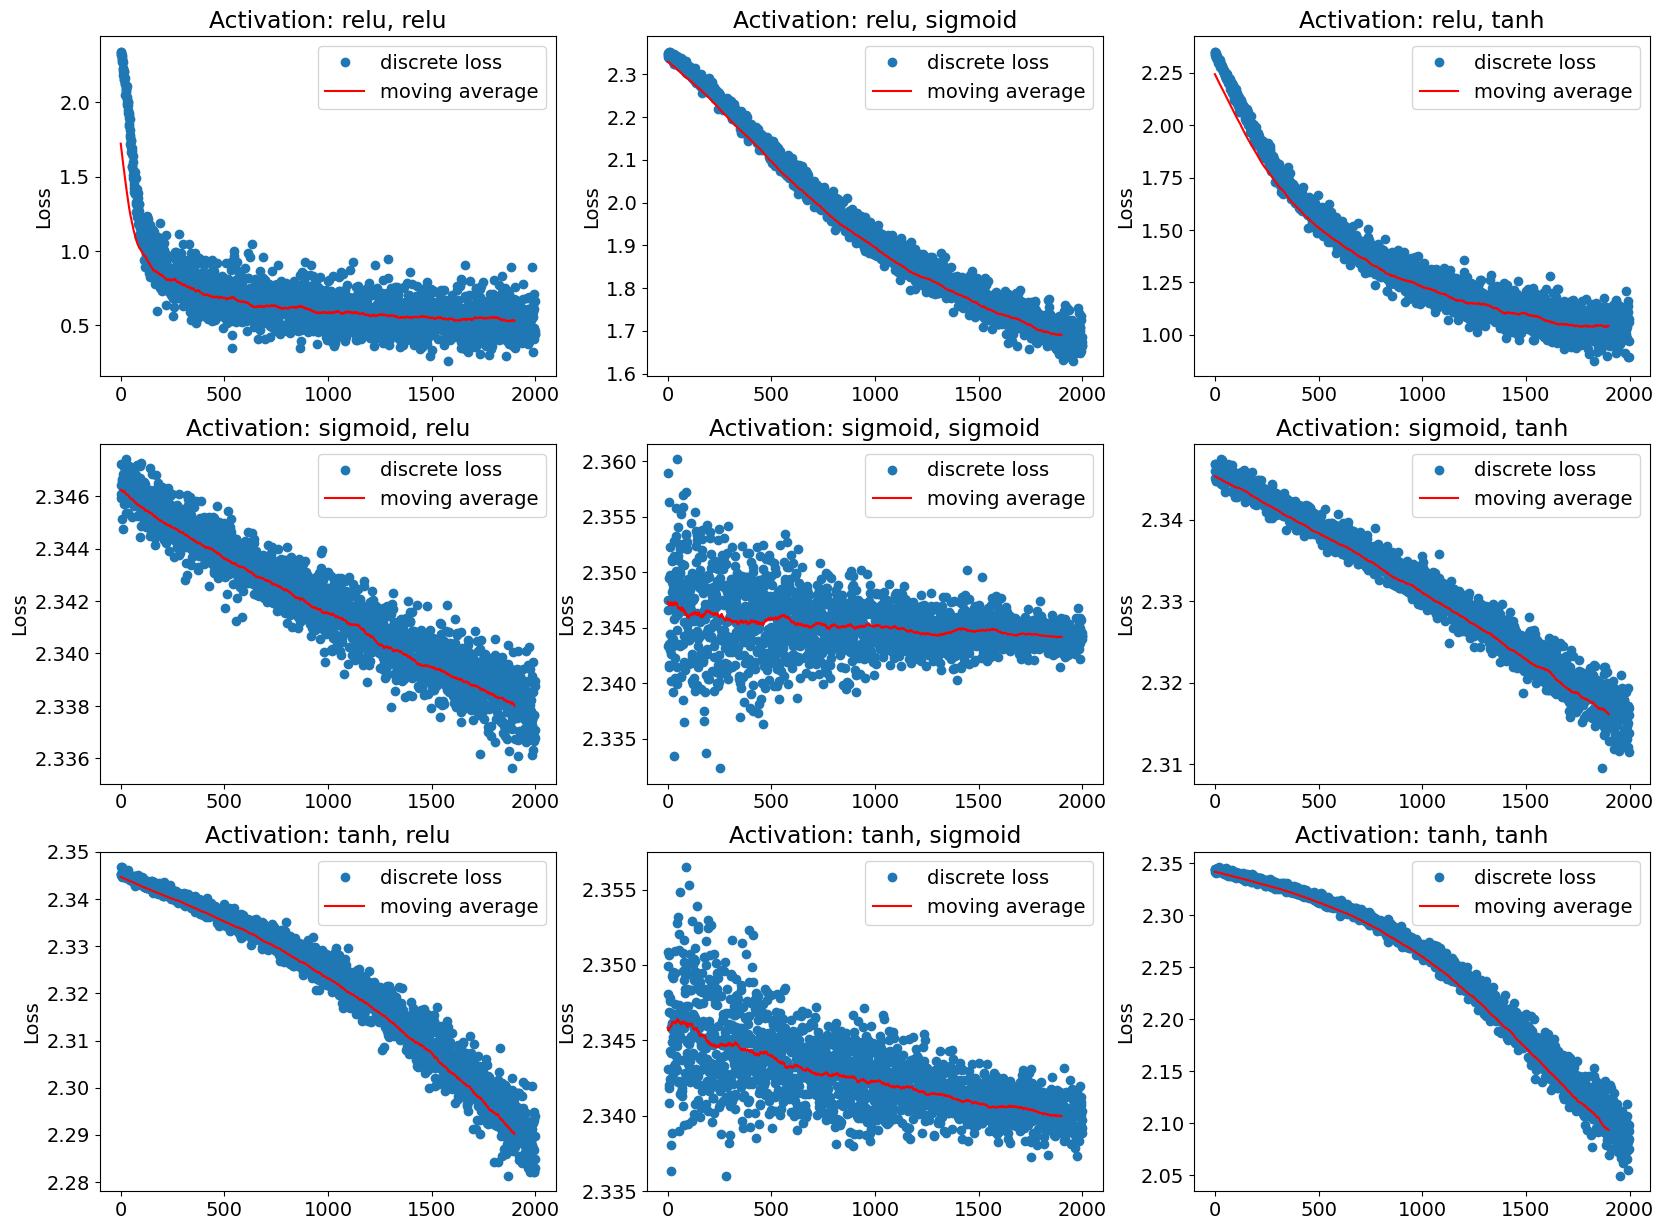
\includegraphics[scale=0.2]{images/activation_loss.png}
    \caption{Loss on different combinations of activation functions}
    \label{fig:activation-loss}
\end{figure}

\begin{figure}[htbp]
    \centering
    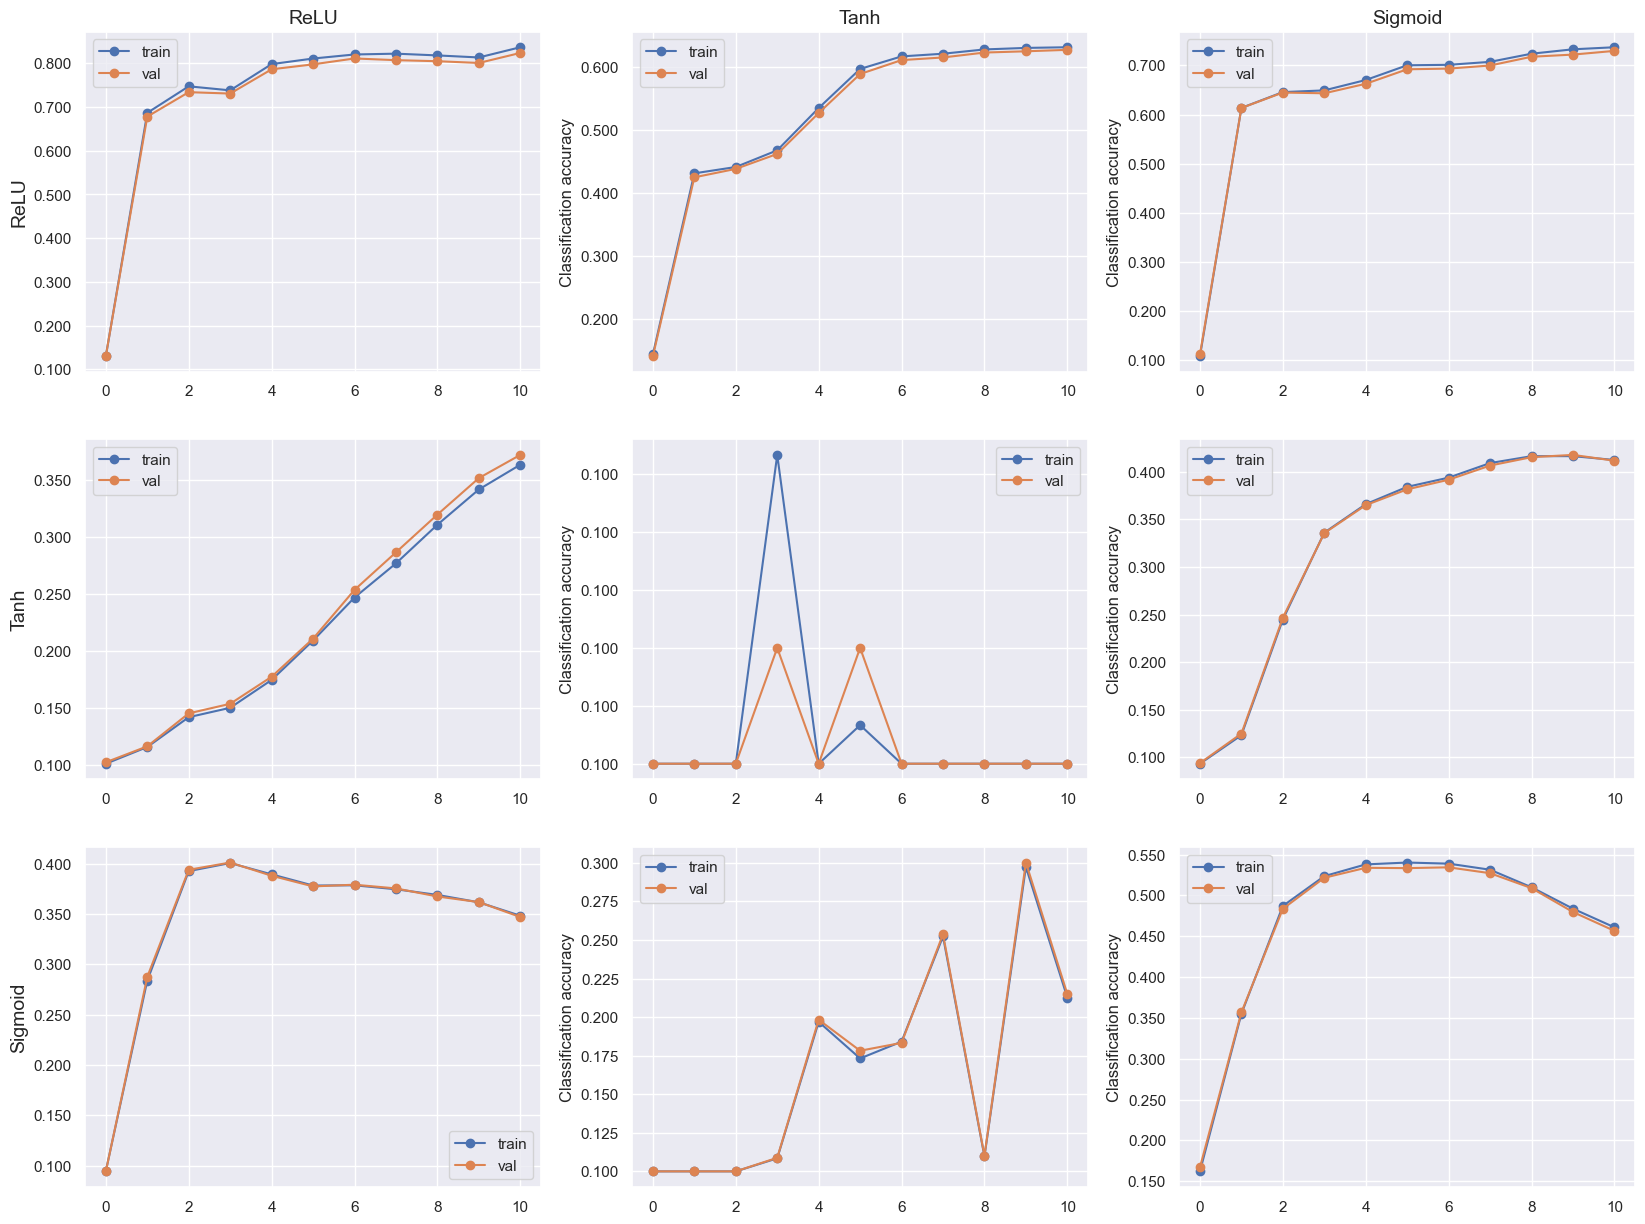
\includegraphics[scale=0.2]{images/activation_acc.png}
    \caption{Accuracy on different combinations of activation functions}
    \label{fig:activation-acc}
\end{figure}

Based on the results, we observe that the top three performing combinations are ['ReLU', 'ReLU'], followed by ['ReLU', 'Sigmoid'], and then ['ReLU', 'Tanh']. Notably, for combinations other than these top three, their loss remains consistently above 2 even after 2000 iterations. The superiority of \texttt{ReLU} over other activation functions is evident, likely attributed to mitigating the gradient vanishing problem present in both \texttt{Tanh} and \texttt{Sigmoid} functions.

Furthermore, it's noteworthy that when \texttt{ReLU} is exclusively applied in the second layer, performance degradation occurs. This observation suggests neural network saturation after the first activation layer if it's not implemented with \texttt{ReLU}. Consequently, we will proceed with the combination ['ReLU', 'ReLU'] in the subsequent sections.


\subsubsection{Grid Search Hyper-parameters}

\subsubsection{Update Rules}

\subsection{Train on Full Dataset}

\section{Load \& Test}

\subsection{Load Pre-trained Model}

\subsection{Evaludate Model on Testing Dataset }

\section{Discussion}



% \section{Appendix}

%     \subsection{Environments preview}

%         The following environments are defined in \textit{tauenvs} package.
		
% 		\subsubsection{Tau environment}

%                 The following code defines the tauenv environment. A custom title can be added to this environment.

% 			\begin{tauenv}[frametitle=Tauenv]
%                     Lorem ipsum dolor sit amet, consectetur adipiscing elit. Sed vestibulum justo quis massa aliquet, ut ultrices quam bibendum.
% 			\end{tauenv}
		
% \begin{lstlisting}[language=TeX, caption=Tauenv environment code.]
% \newmdenv[
% 	backgroundcolor=taublue!22, 					
% 	linecolor=taublue,									
% 	linewidth=0.7pt,
% 	frametitle=\vskip0pt\bfseries,
% 	frametitlerule=false,
% 	frametitlefont=\color{taublue}\bfseries\sffamily,
% 	frametitlealignment=\raggedright,
% 	innertopmargin=3pt,
% 	innerbottommargin=6pt,
% 	innerleftmargin=6pt,
% 	innerrightmargin=6pt,
% 	font=\selectfont,
% 	fontcolor=taublue,									
% 	frametitleaboveskip=8pt,
% 	skipabove=10pt
% ]{tauenv} \end{lstlisting}
		
% 		\subsubsection{Note}

%                 This code defines the note environment.

%   			\begin{note}
%                     Lorem ipsum dolor sit amet, consectetur adipiscing elit. Sed vestibulum justo quis massa aliquet, ut ultrices quam bibendum.
% 			\end{note}
		
% \begin{lstlisting}[language=TeX, caption=Note environment code.]
% \newmdenv[
% 	backgroundcolor=taublue!22, 						
% 	linecolor=taublue,									
% 	linewidth=0.7pt,
% 	frametitle=\vskip0pt\bfseries\notelanguage,
% 	frametitlerule=false,
% 	frametitlefont=\color{taublue}\bfseries\sffamily,
% 	frametitlealignment=\raggedright,
% 	innertopmargin=3pt,
% 	innerbottommargin=6pt,
% 	innerleftmargin=6pt,
% 	innerrightmargin=6pt,
% 	font=\normalfont,
% 	fontcolor=taublue,									
% 	frametitleaboveskip=3pt,
% 	skipabove=10pt
% ]{note} \end{lstlisting}

% 		\subsubsection{Info}

%                 This code defines the info environment.

%     		\begin{info}
%                     Lorem ipsum dolor sit amet, consectetur adipiscing elit. Sed vestibulum justo quis massa aliquet, ut ultrices quam bibendum.
% 			\end{info}
		
% \begin{lstlisting}[language=TeX, caption=Info environment code.]
% \newmdenv[
% 	backgroundcolor=taublue!22, 						
% 	linecolor=taublue,									
% 	linewidth=0.7pt,
% 	frametitle=\vskip0pt\bfseries\infolanguage,
% 	frametitlerule=false,
% 	frametitlefont=\color{taublue}\bfseries\sffamily,
% 	frametitlealignment=\raggedright,
% 	innertopmargin=3pt,
% 	innerbottommargin=6pt,
% 	innerleftmargin=6pt,
% 	innerrightmargin=6pt,
% 	font=\normalfont,
% 	fontcolor=taublue,									
% 	frametitleaboveskip=3pt,
% 	skipabove=10pt
% ]{info} \end{lstlisting}

%     \subsection{Alternative title}

%          You can make the following modification to \textit{tau class} in the \textit{title preferences} section to change the position of the title. This will move the title to the left. 

% \begin{lstlisting}[language=TeX, caption=Alternative title.]
% \renewcommand{\@maketitle}{%
%         \vskip-18pt
%     {\RaggedRight\bfseries\color{taublue}\fontsize{18}{22}\sffamily\selectfont\@title\par}
% 		\vskip8pt
%     {\RaggedRight\normalsize\sffamily\@author\par}
%         \vskip8pt
%     {\RaggedRight\fontsize{7pt}{8pt}\selectfont\@professor\par}
%         \vskip24pt
% }% 
% \end{lstlisting}

%     \subsection{Equation skip value}

%         Play with the value of \verb|\eqskip| until the preferred spacing is set for equations.

% \begin{lstlisting}[language=TeX, caption=Equation skip code.]
% \newlength{\eqskip}\setlength{\eqskip}{6.5pt}
% \expandafter\def\expandafter\normalsize\expandafter{%
%     \normalsize%
%     \setlength\abovedisplayskip{\eqskip}%
%     \setlength\belowdisplayskip{\eqskip}%
%     \setlength\abovedisplayshortskip{\eqskip-\baselineskip}%
%     \setlength\belowdisplayshortskip{\eqskip}%
% }
% \end{lstlisting}
					
% %----------------------------------------------------------

% \addcontentsline{toc}{section}{References}
% \printbibliography

% %----------------------------------------------------------

% \begin{center}
% 	\vskip10pt
% 	Enjoy writing with tau \LaTeX\ class $\blacksmiley$ \\ 
% 	\vskip10pt
% 	\textit{Contact:} \\
% 	\faLink\ \href{https://sites.google.com/view/memo-notess/p%C3%A1gina-principal}{https://sites.google.com/memo-notess} \\
% 	\faEnvelope[regular]\ memo.notess1@gmail.com \\
% 	\faInstagram\ memo.notess\\
% \end{center}

% %----------------------------------------------------------

\end{document}